\documentclass[border=3pt]{standalone}
% Preâmbulo compartilhado pelos diagramas TikZ da aula 6 de IHC (Necessidades e Requisitos)
\usepackage[T1]{fontenc}
\usepackage[utf8]{inputenc}
\usepackage{lmodern}
\usepackage{amsmath}
\usepackage{xcolor}
\usepackage{tikz}
\usetikzlibrary{arrows.meta,angles,quotes,decorations.pathmorphing,calc,
                positioning,shapes.geometric,shapes.misc,backgrounds,fit,
                math}

% Paleta (mesma dos SVGs originais)
% Paleta da disciplina de IHC: acento roxo (#755099), da capa do livro.
% (o nome "dblue" é mantido para não alterar todos os diagramas)
\definecolor{dblue}{HTML}{755099}
\definecolor{dorange}{HTML}{B3541E}
\definecolor{dgreen}{HTML}{4A7C59}
\definecolor{dred}{HTML}{9C4B4B}
\definecolor{dcream}{HTML}{F4F1EA}
\definecolor{dshade}{HTML}{DDD7C9}

% Função gaussiana (não normalizada por padrão de escala visual)
\pgfmathdeclarefunction{gauss}{3}{%
  \pgfmathparse{1/(#3*sqrt(2*pi))*exp(-((#1-#2)^2)/(2*#3^2))}%
}

% Estilos comuns (prefixo d... para não colidir com chaves internas do pgf)
\tikzset{
  >={Stealth[length=2mm]},
  dguide/.style={gray!55, dashed, line width=0.4pt},
  daxis/.style={gray!60, line width=0.7pt, ->},
  dbody/.style={fill=black!3, draw=black!80, line width=1pt},
  dacc/.style={draw=dblue, line width=1pt},
  dlbl/.style={black!55, font=\small},
  dsub/.style={black!45, font=\footnotesize},
  dstate/.style={circle, draw=black!80, fill=dcream, line width=1pt,
                 minimum size=17mm, font=\large, inner sep=1pt},
  dobs/.style={circle, draw=black!80, fill=dshade, line width=1pt,
               minimum size=14mm, font=\large, inner sep=1pt},
  dbox/.style={rounded corners=2pt, draw=black!80, fill=dcream, line width=1pt,
               align=center, inner sep=6pt},
  dop/.style={circle, draw=black!80, fill=white, line width=1pt,
              minimum size=6mm, inner sep=0pt, font=\small},
  dtrans/.style={->, dblue, line width=1pt},
  dmeas/.style={->, dorange, line width=1pt},
  dcurve/.style={line width=1pt, dblue},
  dcurveb/.style={line width=1.4pt, dorange},
}

\begin{document}
\hyphenpenalty=10000 \exhyphenpenalty=10000 \tolerance=9999 \emergencystretch=3em
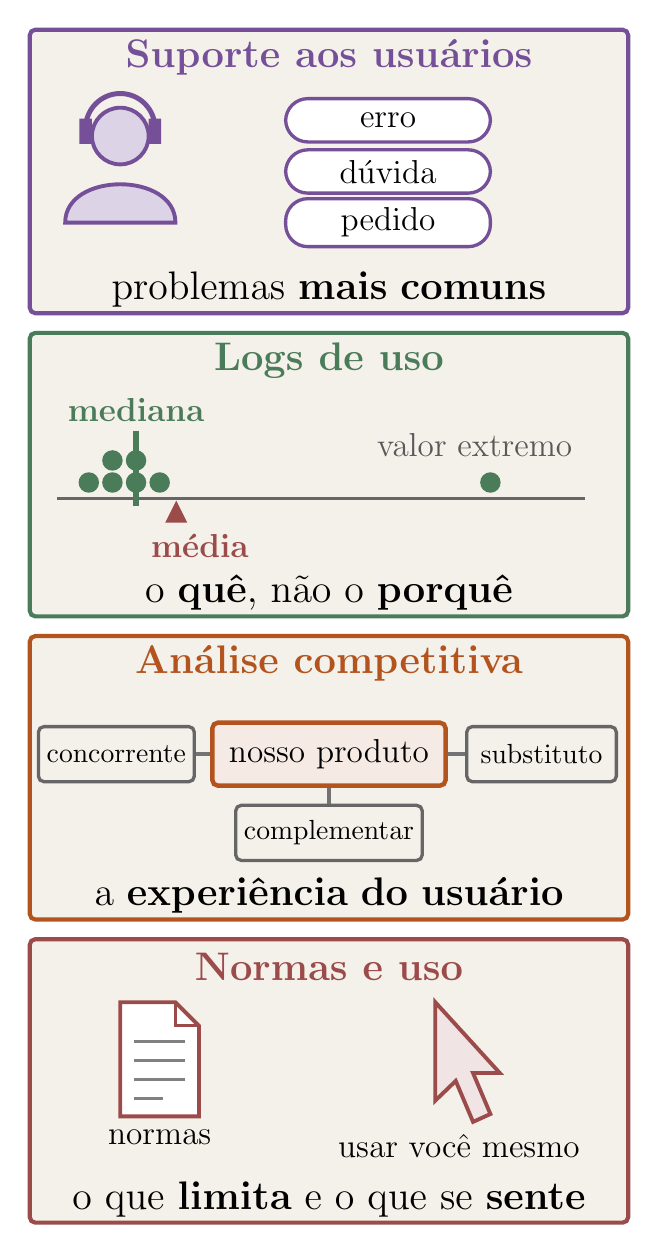
\begin{tikzpicture}[x=1cm,y=1cm]
\node[dbox, draw=dblue, line width=1.5pt, minimum width=7.6cm, minimum height=3.60cm] at (3.80,13.35) {};
\node[font=\Large\bfseries, dblue] at (3.80,14.80) {Suporte aos usuários};
\node[font=\Large, text width=7.2cm, align=center] at (3.80,11.85) {problemas \textbf{mais comuns}};
\fill[dblue!25!white, draw=dblue, line width=1.4pt] (1.15,13.80) circle (0.36);
\fill[dblue!25!white, draw=dblue, line width=1.4pt] (0.45,12.70) .. controls (0.45,13.35) and (1.85,13.35) .. (1.85,12.70) -- cycle;
\draw[dblue, line width=1.8pt] (0.71,13.90) arc (180:0:0.44);
\fill[dblue] (0.63,13.70) rectangle ++(0.16,0.32) (1.51,13.70) rectangle ++(0.16,0.32);
\node[draw=dblue, rounded corners=8pt, fill=white, line width=1.2pt, minimum width=2.6cm, minimum height=0.55cm, font=\large] at (4.55,14.00) {erro};
\node[draw=dblue, rounded corners=8pt, fill=white, line width=1.2pt, minimum width=2.6cm, minimum height=0.55cm, font=\large] at (4.55,13.35) {dúvida};
\node[draw=dblue, rounded corners=8pt, fill=white, line width=1.2pt, minimum width=2.6cm, minimum height=0.55cm, font=\large] at (4.55,12.70) {pedido};
\node[dbox, draw=dgreen, line width=1.5pt, minimum width=7.6cm, minimum height=3.60cm] at (3.80,9.50) {};
\node[font=\Large\bfseries, dgreen] at (3.80,10.95) {Logs de uso};
\node[font=\Large, text width=7.2cm, align=center] at (3.80,8.00) {o \textbf{quê}, não o \textbf{porquê}};
\draw[black!60, line width=1.2pt] (0.35,9.20) -- (7.05,9.20);
\fill[dgreen] (0.75,9.40) circle (0.13);
\fill[dgreen] (1.05,9.40) circle (0.13);
\fill[dgreen] (1.05,9.68) circle (0.13);
\fill[dgreen] (1.35,9.40) circle (0.13);
\fill[dgreen] (1.35,9.68) circle (0.13);
\fill[dgreen] (1.65,9.40) circle (0.13);
\fill[dgreen] (5.85,9.40) circle (0.13);
\draw[dgreen, line width=2pt] (1.35,9.10) -- (1.35,10.05);
\node[font=\large\bfseries, dgreen, anchor=south] at (1.35,10.05) {mediana};
\fill[dred] (1.86,9.17) -- ++(-0.14,-0.28) -- ++(0.28,0) -- cycle;
\node[font=\large\bfseries, dred, anchor=north] at (2.16,8.87) {média};
\node[font=\large, black!65, anchor=south] at (5.65,9.60) {valor extremo};
\node[dbox, draw=dorange, line width=1.5pt, minimum width=7.6cm, minimum height=3.60cm] at (3.80,5.65) {};
\node[font=\Large\bfseries, dorange] at (3.80,7.10) {Análise competitiva};
\node[font=\Large, text width=7.2cm, align=center] at (3.80,4.15) {a \textbf{experiência do usuário}};
\node[dbox, draw=dorange, fill=dorange!12!white, line width=1.6pt, minimum width=2.5cm, minimum height=0.8cm, font=\large] (n) at (3.80,5.95) {nosso produto};
\node[dbox, draw=black!60, line width=1.2pt, minimum width=1.9cm, minimum height=0.7cm, font=\normalsize, inner sep=3pt] (con) at (1.10,5.95) {concorrente};
\draw[black!55, line width=1.2pt] (n) -- (con);
\node[dbox, draw=black!60, line width=1.2pt, minimum width=1.9cm, minimum height=0.7cm, font=\normalsize, inner sep=3pt] (sub) at (6.50,5.95) {substituto};
\draw[black!55, line width=1.2pt] (n) -- (sub);
\node[dbox, draw=black!60, line width=1.2pt, minimum width=1.9cm, minimum height=0.7cm, font=\normalsize, inner sep=3pt] (com) at (3.80,4.95) {complementar};
\draw[black!55, line width=1.2pt] (n) -- (com);
\node[dbox, draw=dred, line width=1.5pt, minimum width=7.6cm, minimum height=3.60cm] at (3.80,1.80) {};
\node[font=\Large\bfseries, dred] at (3.80,3.25) {Normas e uso};
\node[font=\Large, text width=7.2cm, align=center] at (3.80,0.30) {o que \textbf{limita} e o que se \textbf{sente}};
\draw[dred, fill=white, line width=1.4pt] (1.15,1.35) -- (1.15,2.80) -- (1.85,2.80) -- (2.15,2.50) -- (2.15,1.35) -- cycle;
\draw[dred, line width=1pt] (1.85,2.80) -- ++(0,-0.3) -- ++(0.3,0);
\draw[black!50, line width=1pt] (1.33,2.30) -- ++(0.64,0);
\draw[black!50, line width=1pt] (1.33,2.06) -- ++(0.64,0);
\draw[black!50, line width=1pt] (1.33,1.82) -- ++(0.64,0);
\draw[black!50, line width=1pt] (1.33,1.58) -- ++(0.36,0);
\node[font=\large, anchor=north] at (1.65,1.30) {normas};
\draw[dred, fill=dred!15!white, line width=1.4pt] (5.15,2.80) -- (5.15,1.55) -- (5.41,1.80) -- (5.63,1.28) -- (5.85,1.38) -- (5.63,1.90) -- (5.97,1.90) -- cycle;
\node[font=\large, anchor=north] at (5.45,1.25) {usar você mesmo};
\end{tikzpicture}
\end{document}
